\section{1.8. Estudo de caso: discriminação de gênero}

%%%%%%%%%%%%%%%%%%%%%%%%%%%%%%%%%%%%

\subsection{Descrição e dados do estudo}

%%%%%%%%%%%%%%%%%%%%%%%%%%%%%%%%%%%%

\begin{frame}
\frametitle{Discriminação de gênero}

\begin{itemize}
\justifying
\item Em 1972, como parte de um estudo sobre discriminação de gênero, 48 supervisores bancários (homens) receberam o mesmo currículo de um candidato a gerente de uma filial, os supervisores deveriam sugerir se a pessoa deveria ser promovida. 
\justifying
\item Os currículos eram idênticos, exceto que, metade deles o candidato a promoção era do sexo masculino, enquanto a outra metade tinha currículos mostrando que a pessoa era do sexo feminino.
\justifying
\item Foi determinado aleatoriamente quais supervisores receberiam currículos "masculinos" e quais supervisores receberiam currículos "femininos".  
\end{itemize}
\end{frame}
%%%%%%%%%%%%%%%%%%%%%%%%%%%%%%%%%%%%

\begin{frame}
\frametitle{Discriminação de gênero}

\begin{itemize}
\justifying
\item Dos 48 currículos analisados, 35 foram promovidos. 
\justifying
\item O estudo tem como objetivo avaliar se as mulheres são discriminadas injustamente.  
\end{itemize}
\justifying
\dq{Isto é um estudo observacional ou um experimento?} \soln{\onslide<2->{Experimento}}
\justifying
\ct{B.Rosen and T. Jerdee (1974), ``nfluência de estereótipos de papéis sexuais nas decisões de pessoal", J.Applied Psychology, 59:9-14.}

\end{frame}


%%%%%%%%%%%%%%%%%%%%%%%%%%%%%%%%%%%%

\begin{frame}
\frametitle{Dados}
\justifying
\dq{À primeira vista, parece haver uma relação entre promoção e gênero?}

\begin{center}
\begin{tabular}{ll  cc c} 
  		&				& \multicolumn{2}{c}{\textit{Promoção}} \\
\cline{3-4}
							&			& Promovido	& Não Promovido 	& Total	\\
\cline{2-5}
\multirow{2}{*}{\textit{Gênero	}}	&Masculino 		& 21	 	& 3		& 24 	\\
							&Feminino		& 14	 	& 10 	 	& 24 \\
\cline{2-5}
							&Total		& 35		& 13		& 48 \\
\end{tabular}
\end{center}

\pause

\textbf{\% de homens promovidos: $21 / 24 = 0.875$} \\
\textbf{\% de mulheres promovidas: $14 / 24 = 0.583$}

\end{frame}

%%%%%%%%%%%%%%%%%%%%%%%%%%%%%%%%%%%%

\begin{frame}
\frametitle{Prática}
\justifying
\pq{Vimos uma diferença de quase 30\% (29,2\% para ser exato) entre a proporção de currículos de homens e mulheres que seriam promovidos. Com base nessas informações, qual das alternativas abaixo é verdadeira?}
\vspace{-0.5cm}
\small{
\begin{enumerate}[(a)]
\justifying
\item Se fôssemos repetir a experiência, definitivamente veremos que mais mulheres são promovidas. Isso foi o acaso.
\justifying
\item A promoção depende do gênero, os homens têm maior chance de serem promovidos independentemente do currículo, portanto, há discriminação de gênero contra as mulheres nas decisões de promoção. \soln{\only<2>{\red{Talvez}}}
\justifying
\item A diferença na proporção de homens e mulheres a serem promovidos é devido ao acaso, isto não é evidência de discriminação de gênero contra mulheres em decisões de promoção. \soln{\only<2>{\red{Talvez}}}
\justifying
\item As mulheres são menos qualificadas do que os homens, é por isso que menos mulheres são promovidas.

\end{enumerate}
}
\end{frame}

%%%%%%%%%%%%%%%%%%%%%%%%%%%%%%%%%%%%

\subsection{Suposições}

%%%%%%%%%%%%%%%%%%%%%%%%%%%%%%%%%%%%%

\begin{frame}
\frametitle{Duas suposições concorrentes}

\begin{enumerate}
\justifying
\item `` Não há nada acontecendo." \\
\justifying
Promoção e gênero são \hl{independentes}, não há discriminação de gênero, a diferença observada nas proporções é devida, simplesmente,  ao acaso. $\rightarrow$ \hl{Hipótese nula}

\pause
\justifying
\item `` Há algo acontecendo." \\
\justifying
Promoção e gênero são \hl {dependentes}, há discriminação de gênero, a diferença observada nas proporções não se deve ao acaso. $\rightarrow$ \hl{Hipótese alternativa}

\end{enumerate}

\end{frame}

%%%%%%%%%%%%%%%%%%%%%%%%%%%%%%%%%%%%

\begin{frame}
\frametitle{Um julgamento pensado como um teste de hipóteses}

\twocol{0.5}{0.5}
{
\begin{itemize}
\justifying
\item O teste de hipóteses é muito parecido com um julgamento no tribunal.
\justifying
\item $H_0$: Réu é inocente \\
$H_A$: Réu é culpado
\justifying
\item Em seguida, apresentamos as evidências - coletamos dados.

\end{itemize}
}
{
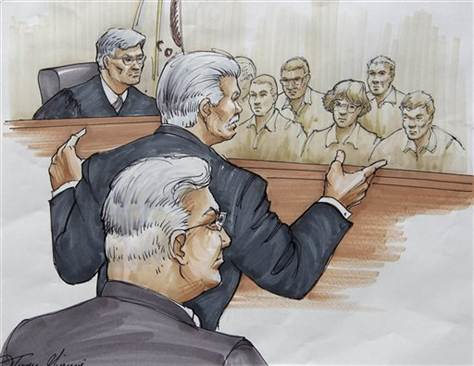
\includegraphics[width=\textwidth]{1-8_gender_discrimination/trial.png}
}

\begin{itemize}
\justifying
\item Então, julgamos as evidências - "Esses dados poderiam ter ocorrido por acaso, se a hipótese nula fosse verdadeira?"
\begin{itemize}
\justifying
\item Se é muito improvável que tenhamos observado determinado conjunto de dados dado que a hipótese nula é verdadeira, as evidências levantam mais do que uma dúvida razoável em nossas mentes. \pause Será que minha suposição inicial, a hipótese nula, é verdade? 
\end{itemize}
\end{itemize}
\end{frame}
%%%%%%%%%%%%%%%%%%%%%%%%%%%%%%%%%%%%

\begin{frame}
\frametitle{Um julgamento pensado como um teste de hipóteses}
\begin{itemize}
\justifying
\item Em última análise, devemos tomar uma decisão. Quão improvável é improvável?

\end{itemize}
\justifying
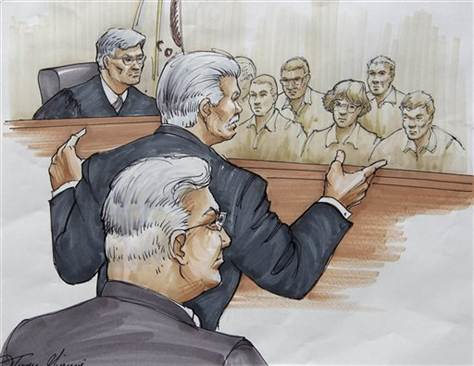
\includegraphics[width=\textwidth]{1-8_gender_discrimination/trial.png}

\ct{Imagem de \webURL{http://www.nwherald.com/_internal/cimg!0/oo1il4sf8zzaqbboq25oevvbg99wpot}.}

\end{frame}

%%%%%%%%%%%%%%%%%%%%%%%%%%%%%%%%%%%%%

\begin{frame}
\frametitle{Um julgamento pensado como um teste de hipóteses (cont.)}

\begin{itemize}
\justifying
\item Se a evidência não for forte o suficiente para rejeitar a suposição de inocência, o júri retorna com um veredicto de "não culpado".
\begin{itemize}
\justifying
\item O júri não diz que o réu é inocente, apenas que não há provas suficientes para condenar.
\justifying
\item O réu pode, de fato, ser inocente, mas o júri não tem como ter certeza.

\end{itemize}
\justifying
\item Estatisticamente falando, não conseguimos rejeitar a hipótese nula.
\begin{itemize}
\justifying
\item Nunca declaramos a hipótese nula como verdadeira, porque simplesmente não sabemos se é verdade ou não.
\end{itemize}

\end{itemize}

\end{frame}

%%%%%%%%%%%%%%%%%%%%%%%%%%%%%%%%%%%%%

\begin{frame}
\frametitle{Um julgamento como teste de hipóteses (cont.)}

\begin{itemize}
\justifying
\item Em um julgamento, o ônus da prova está na acusação.
\justifying
\item Em um teste de hipótese, o ônus da prova está na alegação incomum.
\justifying
\item A hipótese nula é o estado de coisas comum (o status quo), portanto é a hipótese alternativa que consideramos incomum e para a qual devemos coletar evidências.

\end{itemize}

\end{frame}

%%%%%%%%%%%%%%%%%%%%%%%%%%%%%%%%%%%%%

\begin{frame}
\frametitle{Estrutura de teste de hipóteses}

\begin{itemize}
\justifying
\item Começamos com uma \hl {hipótese nula ($ H_0 $)} que representa o status quo.
\justifying
\item Também temos uma hipótese \hl {hipótese alternativa ($ H_A $)} que representa nossa questão de pesquisa, ou seja, o que estamos testando.
\justifying
\item Nós conduzimos um teste de hipótese sob a suposição de que a hipótese nula é verdadeira, simulação (hoje) ou por métodos teóricos (mais tarde no curso).
\justifying
\item Se o resultado do teste sugerem que os dados observados não fornecem evidências convincentes para a hipótese alternativa, nós nos ateremos a hipótese nula. Se os dados fornecerem evidências conta $H_0$, rejeitamos a hipótese nula em favor da alternativa.

\end{itemize}

\end{frame}

%%%%%%%%%%%%%%%%%%%%%%%%%%%%%%%%%%%%

\subsection{Teste via simulação}

%%%%%%%%%%%%%%%%%%%%%%%%%%%%%%%%%%%%%

\begin{frame}
\frametitle{Simulando o experimento da discriminação dado o gênero...}
\justifying
... sob a hipótese de independência, ou seja, que não há diferença entre os dois grupos. \\

\vspace{0.5cm}
\justifying
Se simularmos dados supondo o \hl{modelo aleatório} de independência entre os grupos, e os resultados dessa simulação forem similares com o encontrado na nossa amostra (proporção de homens promovidos 0,87), então podemos determinar que a diferença observadas entre as proporções de currículos promovidos entre homens e mulheres foi simplesmente \hl{devido ao acaso} (promoção e gênero são independentes). \\

\vspace{0.5cm}
\justifying
Se os resultados das simulações baseadas no modelo aleatório não se parecem com os dados observados, então há evidências de que a diferença entre as proporções de arquivos promovidos entre homens e mulheres não foi devida ao acaso, mas \hl{devido a um efeito real de gênero} (promoção e gênero são dependentes).

\end{frame}

%%%%%%%%%%%%%%%%%%%%%%%%%%%%%%%%%%%%

\begin{frame}
\frametitle{Simulando o experimento}
\justifying
\app{
Use um baralho para simular esse experimento.

\begin{enumerate}
\justifying
\item Considere que as cartas de 2-10 representam o grupo \textit{promovido} e as cartas de J-A o \textit{não promovido}.
\begin{itemize}
\justifying
\item Separe os coringas.
\justifying
\item Tire 3 As $\rightarrow$ teremos exatamente 13 cartas restantes nesse grupo (cartas de rosto: A, K, Q, J).
\justifying
\item Pegue uma carta 2 $\rightarrow$ teremos exatamente 35 cartas restantes nesse grupo (cartas numéricas: 2-10).
\end{itemize}
\justifying
\item Embaralhe as cartas e distribua dois grupos de tamanho 24, representando homens e mulheres.
\end{enumerate}
}
\end{frame}
%%%%%%%%%%%%%%%%%%%%%%%%%%%%%%%%%%%%

\begin{frame}
\frametitle{Simulando o experimento}
\app{
\begin{enumerate}
\setcounter{enumi}{2}
\justifying
\item Conte e registre quantos currículos em cada grupo são promovidos (cartas numéricas).
\justifying
\item Calcule a proporção de currículos promovidos em cada grupo e calcule a diferença (homem - mulher), registre esse valor.
\justifying
\item Repita as etapas 2 a 4 várias vezes.

\end{enumerate}
}

\end{frame}

%%%%%%%%%%%%%%%%%%%%%%%%%%%%%%%%%%%%

\begin{frame}
\frametitle{Passo 1}

\begin{center}
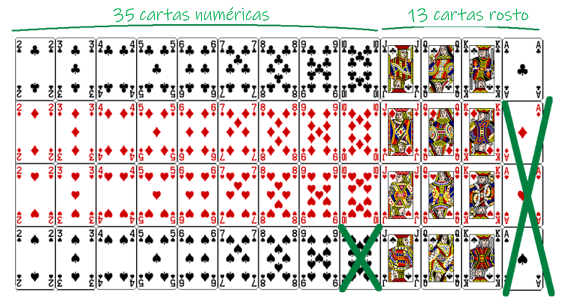
\includegraphics[width=\textwidth]{1-8_gender_discrimination/step1.png}
\end{center}

\end{frame}


%%%%%%%%%%%%%%%%%%%%%%%%%%%%%%%%%%%%

\begin{frame}
\frametitle{Passos 2 - 4}

\begin{center}
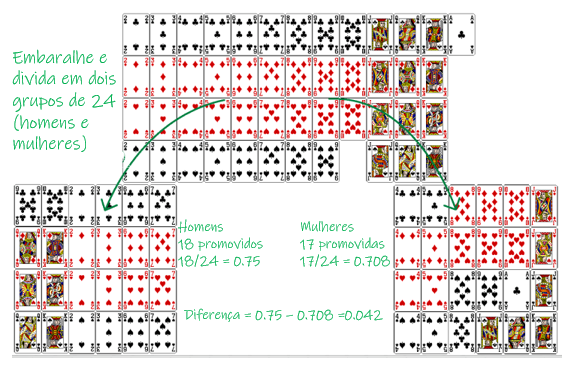
\includegraphics[width=\textwidth]{1-8_gender_discrimination/step2.png}
\end{center}

\end{frame}


%%%%%%%%%%%%%%%%%%%%%%%%%%%%%%%%%%%%

\subsection{Verificando a independência}

%%%%%%%%%%%%%%%%%%%%%%%%%%%%%%%%%%%%

\begin{frame}
\frametitle{Prática}
\justifying
\pq{Os resultados da simulação que você acabou de executar fornecem evidências convincentes de discriminação de gênero contra as mulheres, ou seja, dependência entre gênero e decisões de promoção?}

\begin{enumerate}[(a)]
\justifying
\item Não, os dados não fornecem evidências convincentes para a hipótese alternativa, portanto, não podemos rejeitar a hipótese nula de independência entre gênero e promoção. A diferença observada entre as duas proporções foi devida ao acaso.
\justifying
\solnMult{Sim, os dados fornecem evidências convincentes para a hipótese alternativa de discriminação de gênero contra as mulheres nas decisões de promoção. A diferença observada entre as duas proporções foi devida a um efeito real de gênero.}
\end{enumerate}

\end{frame}

%%%%%%%%%%%%%%%%%%%%%%%%%%%%%%%%%%%%

\begin{frame}
\frametitle{Simulações usando software}
\justifying
Usamos um software para gerar as simulações descritas anteriormente. Consulte o livro da disciplina 
\href{https://www.ufrgs.br/probabilidade-estatistica/livro/cpt1/ch1_intro.html#caseStudyGenderDiscrimination}{https://www.ufrgs.br/probabilidade-estatistica/livro/cpt1/ch1 intro.html#caseStudyGenderDiscrimination} e aprenda como fazer o gráfico abaixo utilizando o R.

O gráfico de pontos abaixo mostra a distribuição das diferenças simuladas nas taxas de promoção com base em 100 simulações.

\begin{center}
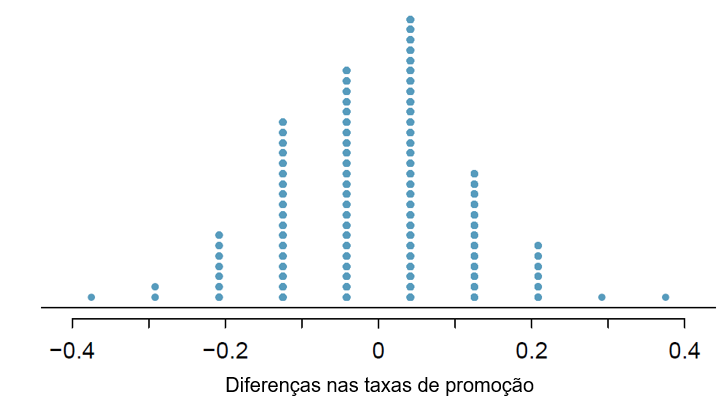
\includegraphics[width=0.7\textwidth]{1-8_gender_discrimination/discRandDotPlot.png}
\end{center}

\end{frame}

%%%%%%%%%%%%%%%%%%%%%%%%%%%%%%%%%%%%%

